%~~~~~~~~~~~~~~~~~~~~~~~~~~~~~~~~~~~~~~~~~~~~~~~~~~~~~~~~~~~~~~~~~~~~~~~
\section{\emph{Count-Min Sketch}}\label{sec:countmin}
%~~~~~~~~~~~~~~~~~~~~~~~~~~~~~~~~~~~~~~~~~~~~~~~~~~~~~~~~~~~~~~~~~~~~~~~

\emph{Count-Min Sketch} é uma estrutura probabilística, descrita por Cormode e Muthukrishnan \cite{cormode2005improved}, que permite representar um vetor implicitamente e incrementalmente e estimar consultas sobre ele. 

Esta estrutura mostra-se importante em casos onde o vetor representado não caberia em memória, sendo aceitáveis resultados probabilísticos para consultas específicas.

Em especial, \emph{Count-Min Sketch} e suas variantes permitem estimar o valor em índices e intervalos específicos do vetor, bem como o produto escalar entre diferentes vetores.

Estas operações ajudam a resolver muitos problemas relacionados à análise de fluxos de dados. Em especial, ao representar os elementos de um multiconjunto de inteiros como os índices do vetor $A$, e suas frequências como os valores, é possível utilizar a consulta de intervalo para estimar os percentis do multiconjunto original.

\subsection{Definição}


O objetivo de \emph{Count-Min Sketch} é representar um vetor $A$,  definido incrementalmente através de operações de atualização na forma de pares ordenados $(i, c)$, que representam um acréscimo de $c$ unidades na i-ésima posição do vetor. Isto é $A[i] \gets A[i] + c$. 

O vetor e suas atualizações não precisam ser mantidos em memória. A estrutura permite a qualquer momento, efetuar consultas sobre parâmetros do vetor original, respondidas probabilisticamente. Em especial, descreveremos nesta seção o processo para responder as seguintes consultas:

\begin{itemize}
  \item Para um índice $i$, o valor $A[i]$;
  \item Para vetores $A$ e $B$, o produto escalar $A \cdot B$.
\end{itemize}

\emph{Count-Min Sketch} funciona de forma similar a um filtro de Bloom com contagem, entretanto, em vez de apenas um vetor, a estrutura utiliza uma matriz $M[1..m, 1..k]$, onde cada coluna corresponde a uma função \emph{hash}.

A atualização parte de um par ordenado $(i, c)$, representando um incremento de valor $c$ na $i$-ésima posição do vetor implícito $A$. O algoritmo consiste em incrementar na matriz todas as posições referenciadas pelos hashs calculados em cada um dos seus respectivos vetores (Algoritmo~\ref{alg:countminupdate}). 

\begin{algorithm}
\linespread{1}\selectfont
\caption{Atualiza Count-Min}
\label{alg:countminupdate}
\begin{algorithmic}[1]
\Procedure{Atualizar}{$i$, $c$}
    \For{$j \gets  1 \textrm{ to } k$}
        \State $M[h_j(i), j] \gets M[h_j(i), j] + c$
	\EndFor
\EndProcedure
\end{algorithmic}
\end{algorithm}

A consulta por valor se dá obtendo o mínimo entre todas as células referenciadas pelas funções \emph{hash}  (Algoritmo~\ref{alg:countminquery}).

\begin{algorithm}
\linespread{1}\selectfont
\caption{Estima valor de $A[i]$}
\label{alg:countminquery}
\begin{algorithmic}[1]
\Function{Estimar}{$i$}
    \State $resultado \gets \infty$ 
    \For{$j \gets  1 \textrm{ to } k$}
        \State $resultado \gets \min(resultado, M[h_j(i), j])$
	\EndFor
	\Return $resultado$
\EndFunction
\end{algorithmic}
\end{algorithm}

A Figura~\ref{fig:countmin1} exemplifica os dois processos anteriores.

\begin{figure}[!htbp]
  \centering
  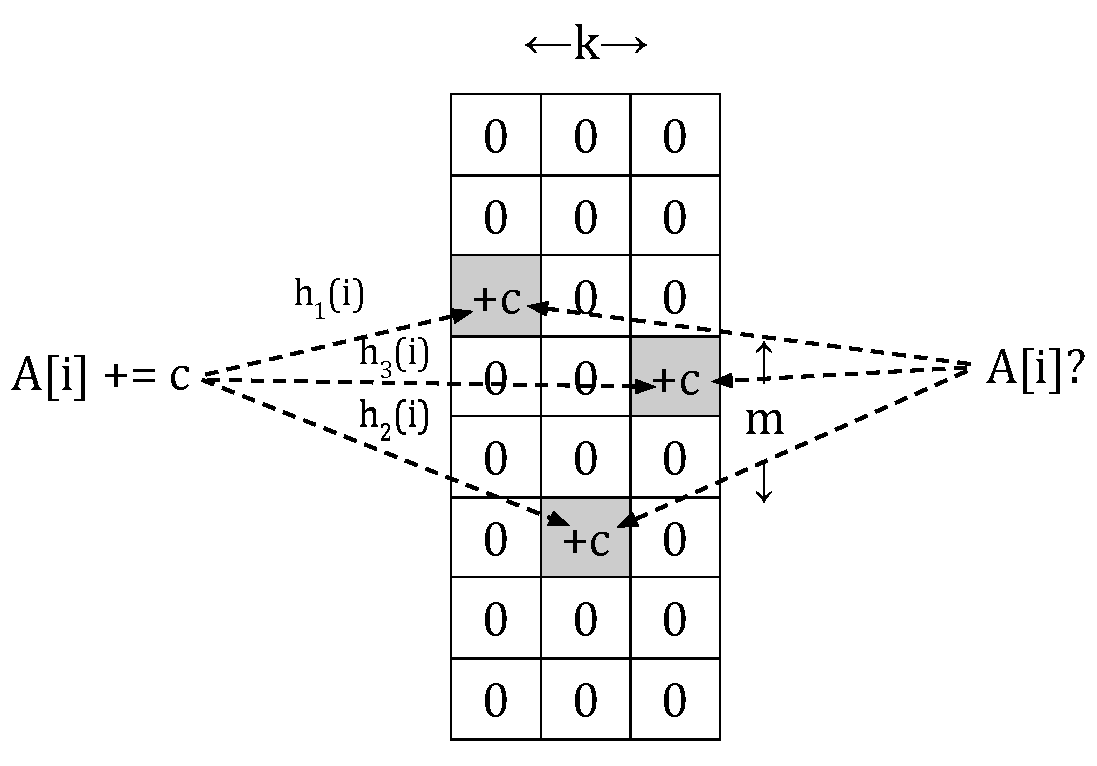
\includegraphics[scale=0.45]{files/countmin1.pdf}
  \caption{Atualização e consulta em um \emph{Count-Min Sketch}}
  \label{fig:countmin1}
\end{figure}

Percebe-se intuitivamente que, no caso de $\forall_i A[i] \leq 0$ no momento da consulta, o valor estimado pela mesma nunca é menor do que o valor real do elemento, isto é: $A[i] \leq \widehat{A[i]}$. Este resultado é importante, pois representa muitos casos reais de uso, como contagem de acessos de usuários ou monitoramento de uso e liberação de recursos compartilhados.

Dadas duas matrizes \emph{Count-Min} $M_A[1..m, 1..k]$ e $M_B[1..m, 1..k]$ representando, respectivamente, vetores implicitos $A$ e $B$, é possível estimar o produto escalar $A \cdot B$ obtendo o mínimo valor entre os produtos escalares das respectivas colunas nas duas matrizes, como mostrado no Algoritmo~\ref{alg:countminscalar}.

\begin{algorithm}
\linespread{1}\selectfont
\caption{Estima $A \cdot B$}
\label{alg:countminscalar}
\begin{algorithmic}[1]
\Function{Produto-Escalar}{$M_A$, $M_B$}
    \State $resultado \gets \infty$ 
    \For{$i \gets  1 \textrm{ to } k$}
        \State $soma \gets 0$ 
        \For{$j \gets  1 \textrm{ to } m$}
            \State $soma \gets soma + M_A[i, j] \cdot M_B[i, j]$
        \EndFor
        \State $resultado = \min(resultado, soma)$
	\EndFor
	\Return $resultado$
\EndFunction
\end{algorithmic}
\end{algorithm}

De forma análoga à consulta pontual, caso ambos os vetores tenham apenas elementos não-negativos, vale que $A \cdot B \leq \widehat{A \cdot B}$.

\subsection{Exemplo}\label{sec:countmin:example}


\subsection{Estimativa do erro}

Em \cite{cormode2005improved} é mostrado que a escolha dos parâmetros $m$ e $k$ se dá de forma a definir $\epsilon$ (o fator de erro) e $\delta$ (a confiança do erro). Isto é, dados $m = \lceil e/\epsilon \rceil$ e $k = \lceil \ln(1/\delta) \rceil$, é possível mostrar que o erro da estimativa $\widehat{A[i]}$ se dá por um fator de $\epsilon$. Mais especificamente, se $\forall_i A[i] \geq 0$,
\[
A[i] \leq \widehat{A[i]} \leq A[i] + \epsilon \lVert A \rVert_1
\]
com probabilidade inferior a $1 - \delta$.

Para demonstrar este resultado, precisamos introduzir uma variável aleatória $I_{h,i,j}$, que representa, para cada função \emph{hash}, incidência de dois índices distintos em $A$ na mesma linha na matriz. Isto é, para cada função $h$
\[
    I_{h,i,j} = \begin{cases} 
        1 & \text{se}\ i \neq j \wedge h(i) = h(j) \\
        0 & \text{caso contrário} \\
    \end{cases}
\]

Perceba que $I_{h,i,j}$ é uma variável de Bernoulli, portanto, 
\[
\text{E}[I_{h,i,j}] = \Pr[h(i) = h(j)] = \frac{1}{m} \leq \frac{\epsilon}{e}
\]

Definimos também uma variável $X_{h, i}$, que representa, para cada função \emph{hash}, o somatório de elementos em $A$ (exceto o próprio índice $i$) que foram adicionados na mesma célula da matriz que $A[i]$, isto é
\[
    X_{h, i} = \sum_{j=1}^{n} I_{h,i,j} A[j]
\]

A variável $X_{h, i}$ pode ser interpretada como o erro na estimativa para cada função \emph{hash}, isto é $M[h_q(i), q] = A[i] + X_{h_q, i}$. Como todo $A[i]$ é não-negativo, $X_{h, i}$ também é não-negativo, portanto $\widehat{A[i]} \geq A[i]$. Além disso, pela linearidade da expectativa, 
\[
    \text{E}[X_{h, i}] = \text{E} \left[ \sum_{j=1}^{n} I_{h,i,j} A[j] \right] =  \text{E}[I_{h,i,j}] \sum_{j=1}^{n}A[j] \leq \frac{\epsilon}{e} \lVert A \rVert_1
\]

Para provar o limite superior, analisaremos a probabilidade de uma estimativa estar acima deste limite. Para isso, todas as funções \emph{hash} precisam gerar estimativas acima do limite, ou seja
\begin{align*}
    \Pr\left[ \widehat{A[i]} > A[i] + \epsilon \lVert A \rVert_1\right] 
    &= \Pr\left[ \forall_q^k M[h_q(i), k] > A[i] + \epsilon \lVert A \rVert_1 \right] \\
    &= \Pr\left[ \forall_q^k A[i] + X_{h_q,i} > A[i] + \epsilon \lVert A \rVert_1 \right] \\
    &= \Pr\left[ \forall_q^k X_{h_q,i} > e \text{E} [X_{h_q,i}] \right] \\
    &= (\Pr\left[ X_{h_q,i} > e \text{E} [X_{h_q,i}] \right])^k
\end{align*}
e, pela desigualdade de Markov,
\[
    \Pr\left[ \widehat{A[i]} > A[i] + \epsilon \lVert A \rVert_1 \right] < \frac{1}{e^k} \leq \delta \\
\]

Ou seja, para o caso $\forall_i A[i] \geq 0$, a probabilidade da estimativa $\widehat{A[i]}$ não ultrapassar o limite superior definido é menor que $1 - \delta$.

É possível utilizar uma variante do algoritmo para o caso geral, onde $A[i]$ pode assumir valores negativos no momento da estimativa. Neste caso, utiliza-se a mediana como estimativa no lugar do mínimo. É possível então demonstrar que
\[
A[i] - 3 \epsilon \lVert A \rVert_1 \leq \widehat{A[i]} \leq A[i] + 3 \epsilon \lVert A \rVert_1
\]
com probabilidade $1 - \delta^{1/4}$. Basta observar que dado que $M[h_q(i), q] = A[i] + X_{h_q, i}$, segue
\[
\text{E}\left[ |M[h_q(i), q] - A[i]| \right] = \text{E}[X_{h_q,i}] \leq \frac{\epsilon}{e} \lVert A \rVert_1
\]

Aplicando novamente a desigualdade de Markov, mostra-se que a probabilidade da estimativa de cada função \emph{hash} estar errada por um valor absoluto maior que $3\epsilon \lVert A \rVert_1$ é menor que $1/3e$. Como estamos obtendo a mediana de $\lceil \ln(1/\delta) \rceil$ estimadores, a probabilidade de pelo menos metade deles estar acima do limite de erro que pretendemos provar, pelo limite de Chernoff, é menor que $\delta^{1/4}$.

Por fim, o erro esperado para a estimativa do produto escalar entre vetores se dá pela desigualdade
\[
    A \cdot B \leq \widehat{A \cdot B} \leq A \cdot B + \epsilon \lVert A \rVert_1 \lVert B \rVert_1
\]

Para esta demonstração, definimos $(\widehat{A \cdot B})_q$ como a estimativa do produto escalar considerando apenas a coluna $q$ da matriz. Pela construção da matriz, pode-se dizer que
\[
    (\widehat{A \cdot B})_q = A \cdot B + \sum_{i,j} I_{h_q,i,j} \cdot A[i] \cdot B[j] 
\]

Como todo ambos $A$ e $B$ possuem apenas elementos não-negativos, é fácil mostrar que tanto os valores de $(\widehat{A \cdot B})_q$ como a estimativa final (por consequência) são maiores que o valor do produto escalar $A\cdot B$. Além disso,
\begin{align*}
    E\left[ (\widehat{A \cdot B})_q - A \cdot B \right] 
    &= E\left[ \sum_{i,j} I_{h_q,i,j} \cdot A[i] \cdot B[j]  \right] \\
    &= \sum_{i,j} E\left[ I_{h_q,i,j} \right] \cdot A[i] \cdot B[j] \\
    &\leq \frac{\epsilon}{e}   \lVert A \rVert_1 \lVert B \rVert_1
\end{align*}

Assim, a probabilidade de todas as funções \emph{hash} produzirem estimativas acima do limite é dada por
\begin{align*}
    \Pr\left[ \widehat{A \cdot B} > A \cdot B + \epsilon \lVert A \rVert_1 \lVert B \rVert_1 \right] 
    &= \Pr\left[ \forall_q^k (\widehat{A \cdot B})_q -  A \cdot B > \epsilon \lVert A \rVert_1 \lVert B \rVert_1 \right] \\
    &= \Pr\left[ \forall_q^k (\widehat{A \cdot B})_q -  A \cdot B > e  E\left[ (\widehat{A \cdot B})_q - A \cdot B \right]  \right] \\
    &= \left(\Pr\left[ (\widehat{A \cdot B})_q -  A \cdot B > e  E\left[ (\widehat{A \cdot B})_q - A \cdot B \right]  \right]\right)^k \\
\end{align*}

logo, utilizando a desigualdade de Markov,
\[
    \Pr\left[ \widehat{A \cdot B} > A \cdot B + \epsilon \lVert A \rVert_1 \lVert B \rVert_1 \right] < \frac{1}{e^k} \leq \delta \\
\]

Perceba que este é um resultado compatível e mais geral à consulta de ponto no vetor. Neste caso, bastaria utilizar um vetor $B$, com apenas o índice $i$ contendo o valor $1$. Assim, o produto escalar deste com um vetor $A$ arbitrário seria equivalente a obter $A[i]$.

\subsection{Consultas de intervalo}

É possível utilizar \emph{Count-Min Sketch} para consultas de intervalo $Q(a, b) = \sum_{i=a}^b A[i]$ em um vetor $A[0..n-1]$. A ideia trivial seria fazer a estimativa de todos os valores $A[i]$ no intervalo selecionado. Porém, esta estratégia acumula erro proporcional ao tamanho do intervalo.

Uma outra estratégia envolve manter não apenas um, mas $\log_2 n$ matrizes $M_y, 0 \leq y < \log_2 n$, representando implicitamente vetores $A_y$, onde cada $A_y[i] = \sum_{j=0}^{2^y-1} A[i+j]$. Isto permite que qualquer consulta nos intervalos em $[0, n)$ seja efetuada com no máximo $2 \log_2 n$ consultas nas matrizes subjacentes. A Figura~\ref{fig:countmin2} exemplifica uma dessas consultas.

\begin{figure}[!htbp]
  \centering
  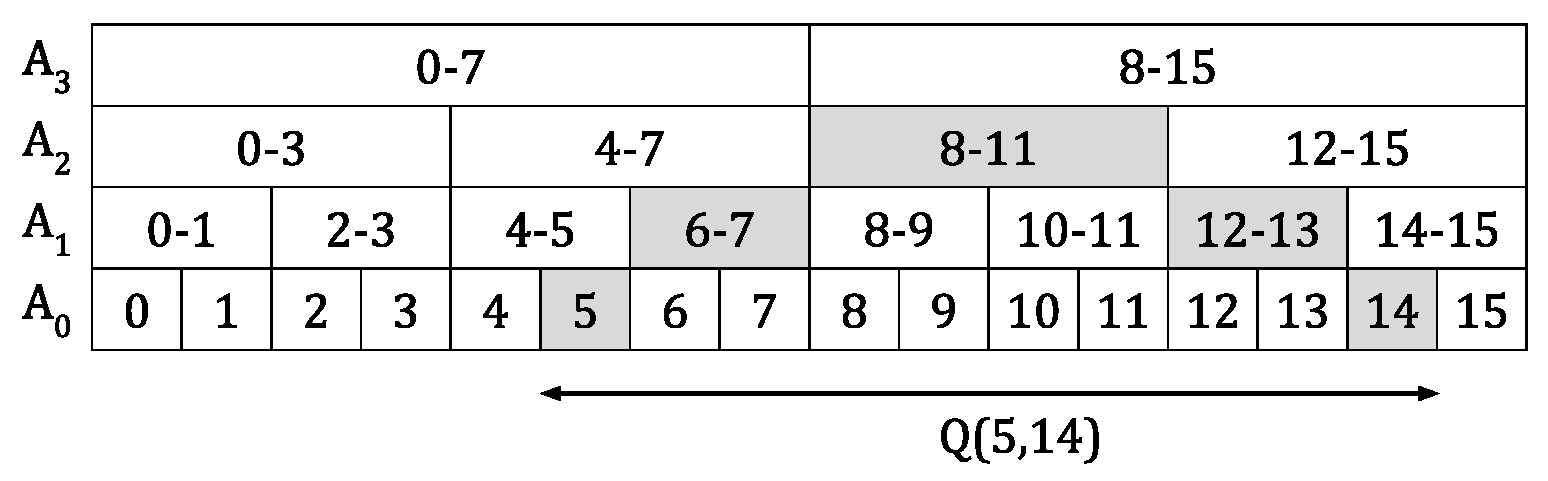
\includegraphics[scale=0.45]{files/countmin2.pdf}
  \caption{Consulta de intervalo $Q(5, 14)$ para $n=16$}
  \label{fig:countmin2}
\end{figure}

A atualização envolve em, ao receber uma tupla $(i, c)$, atualizar cada uma das matrizes. Porém o índice utilizado em cada matriz é diferente. Seja $i_y$ o índice usado para atualizar a matriz $M_y$, todos os bits $i_y$ deve ser iguais aos de $i$, exceto os $y$ últimos, que devem ser zero.

Por exemplo, para atualizar $i=7$ num vetor com $n=16$, as seguinte posições devem ser atualizadas nos vetores implícitos: $i_0 = 7$, $i_1=6$, $i_2=4$ e $i_3=0$. O Algoritmo~\ref{alg:countminrangeupdate} mostra como se dá essa atualização.

\begin{algorithm}
\linespread{1}\selectfont
\caption{Atualiza Count-Min para busca por intervalo}
\label{alg:countminrangeupdate}
\begin{algorithmic}[1]
\Procedure{Atualizar}{$i$, $c$}
    \For{$y \gets 0 \textrm{ to } \log_2 n - 1$}
        \State $i_y \gets i \textrm{ com os } y \textrm{ bits menos significativos desligados}$
        \For{$j \gets  1 \textrm{ to } k$}
            \State $M_y[h_j(i_y), j] \gets M_y[h_j(i_y), j] + c$
    	\EndFor
	\EndFor
\EndProcedure
\end{algorithmic}
\end{algorithm}

A consulta envolve decidir e estimar os valores para os sub-intervalos canônicos que compõem o intervalo de busca. A decomposição em sub-intervalos canônicos pode ser feita de forma gulosa, em cada passo procurando o maior sub-intervalo que seja prefixo do intervalo atual. Para os fins do algoritmo, o mais importante é encontrar qual vetor $A_y$ representa o intervalo em questão. O Algoritmo~\ref{alg:countminrangequery} mostra como funciona o processo de consulta.

\begin{algorithm}
\linespread{1}\selectfont
\caption{Estima o somatório dos elementos no intervalo}
\label{alg:countminrangequery}
\begin{algorithmic}[1]
\Function{Estimar-Intervalo}{$a$, $b$}
    \State $soma \gets 0$
    \While{$a \leq b$}
        \State $y \gets $ maior índice de vetor $A_y$ que representa algum prefixo de $[a, b]$.
        \State $minimo \gets \infty$
        
        \For{$j \gets  1 \textrm{ to } k$}
            \State $minimo \gets \min(minimo, M_y[h_j(a), j])$
    	\EndFor
    	
    	\State $soma \gets soma + minimo$
    	\State $a \gets a + 2^y$
    \EndWhile
    \Return $soma$
\EndFunction
\end{algorithmic}
\end{algorithm}

Ainda seguindo o trabalho em \cite{cormode2005improved}, é possível mostrar que o erro desta estimativa é dado por
\[
    A[a..b] \leq \widehat{A[a..b]} \leq A[a..b] + 2  \epsilon \log_2 n \lVert A \rVert_1
\]
com probabilidade $1-\delta$.

O princípio que rege este erro é o mesmo da consulta pontual. Neste caso, a ideia é mostrar que o erro de cada estimativa (somatório de até $2\log_2 n$ observações independentes de $X_{h,i}$) tem valor esperado $2 \log_2 n (\epsilon/e) \lVert A \rVert_1$. Assim, aplicando a mesma desigualdade de Markov temos o resultado descrito acima. 

É importante notar que na prática, o erro pode ser menor para intervalos cujos limites possuam um número menor de bits ligados, pois seriam necessários menos sub-intervalos para compor o intervalo da consulta.

\subsection{Aplicações}

A estrutura \emph{Count-Min Sketch} permite a representação de vetores arbitrários sem o custo de mantê-los inteiramente em memória. Isto pemite a utilização de diversos algoritmos clássicos que seriam custosos em uma situação de restrição de recursos, mas que não sofreriam tanto em trocar acurácia das respostas por um uso mais controlado de memória.

\begin{description}

\item[Bioinformática:]

Em \cite{zhang2014these} é mostrado um caso onde a estrutura \emph{Count-Min sketch} é usada para manter a contagem de \emph{k-mers} (subsequências de K bases nitrogenadas em sequências de DNA). Estas frequências são usadas para alimentar outros algoritmos, que passam então a atuar de forma probabilística. O uso de estruturas probabilísticas neste caso é importante para aliviar o uso de memória para representar conjuntos de dados que não raramente chegam a dezenas de bilhões de registros.

\item[Segurança:]

Muitos equipamentos de segurança possuem uma quantidade limitada de recursos computacionais. Isto torna atrativo o uso de estruturas de \emph{sketch} para manter informações críticas em tempo real. Em \cite{salem2008novel} é descrito um mecanismo que usa \emph{Count-Min sketch} para verificar se uma certa combinação de parâmetros de conexão exibe uma frequência muito superior à média, o que pode ser um sinal de ataque.

Além disso, em \cite{schechterpopularity}, pesquisadores da Microsoft apresentam um mecanismo para manter uma estrutura com a frequência de senhas para invalidar senhas muito comuns, aumentando a segurança dos sistemas. A vantagem de usar \emph{Count-Min} neste caso é capacidade de armazenar a frequência de uma senha sem manter a senha em si na estrutura.

\item[Bancos de Dados:]

Um uso prático para a estrutura \emph{Count-Min sketch} é a estimativa de joins relacionais em bancos distribuídos \cite{cormode2005improved,rusu2007statistical}. Neste uso, seria computada a estrutura para o vetor de frequências dos diferentes valores que um certo atributo pode ter e, apenas transferindo o \emph{sketch} é possível estimar a cardinalidade do join, através da estimativa do produto escalar entre os dois vetores.

\item[Sistemas distribuídos:]

Encontrar certos elementos muito frequentes num fluxo de dados tem muitas aplicações práticas, como detecção de cenários de erros persistentes. Entretanto, algoritmos determinísticos para esse problema geralmente envolvem manter um contador para cada elemento distinto no conjunto. Utilizando a estrutura \emph{Count-Min sketch} é possível derivar um algoritmo que estima com alta probabilidade quais são os elementos mais frequentes \cite{zhao2006finding}. Este algoritmo ainda tem a vantagem de poder ser executado de forma distribuída, pela própria natureza da estrutura de dados.




\end{description}

\subsection{Resultados experimentais}\label{sec:count:experiments}

Com o objetivo de testar as previsões teóricas sobre a estrutura \emph{Count-Min sketch}, realizamos experimentos que verificam empiricamente os erros descritos anteriormente.

Cada teste usou uma variação do mesmo conjunto de daods composto por todas as obras de Shakespeare (42 obras, 964410 palavras, 23704 distintas). Em todos os casos, a família de funções \emph{hash} utilizada foi MurmurHash 3 \cite{appleby2012murmur}, de 32 bits. Várias funções foram geradas, usando sementes diferentes. Para todos os testes, fixamos $k=3$, o que resulta em uma confiança acima de 95\% para todas as estimativas

No primeiro teste, todas as palavras em todas as obras foram inseridas em \emph{sketches} com $m$ variando entre 128 e 4096. Depois, foram estimados as frequências de cada uma das palavras distintas bem como o erro relativo à norma $\lVert A \rVert_1$ do vetor. O resultado (média e percentil 99), bem como a previsão teórica, podem ser observado na Figura~\ref{fig:countmin_result}.

\begin{figure}[!htbp]
\centering
\scalebox{0.80}{\begin{tikzpicture}[
            declare function = {
                p(\m) = min(e/\m, 0.01);
            }
        ]
    	\begin{axis}[
    	    %height=7cm, width=13cm,
    	    scaled ticks=false, 
            grid=both,
            ylabel={erro relativo a $\lVert A \rVert_1$},
            xlabel=tamanho de cada vetor ($m$),
    		yticklabel=\pgfmathparse{100*\tick}\pgfmathprintnumber{\pgfmathresult}\,\%,
    		ymin=0,ymax=0.003,
    		xmin=0, xmax=4096, 
    		legend columns=1, 
    		legend style={legend pos=outer north east,}
        ]
    
        \addplot[line width=15pt,domain=0:1,samples=30,color={rgb:black,1;white,1},opacity=0.4]{0.01};
    
        \addplot[name path=line3, line width=0pt,domain=1:4096,samples=40,opacity=0.0,forget plot]{p(x)};
        \addplot[name path=line4, line width=15pt,domain=1:4096,samples=30,opacity=0.0, forget plot]{0};
    
    	\addplot[fill={rgb:black,1;white,1},fill opacity=0.40,forget plot] fill between[ of = line3 and line4];
    
    	\addplot[line width=1pt, mark=*,black,smooth, mark options={scale=0.75}] table[x=k,y=mean] {files/countmin.txt};
    	\addplot[dashed,line width=1pt, mark=none,black,smooth, mark options={scale=0.75}] table[x=k,y=p99] {files/countmin.txt};
    	\legend{esperado ($\delta = 0.05$), observado (média), observado ($P_{99}$)};

    	\end{axis}
    \end{tikzpicture}}
\caption{Distribuição de similaridades entre pares de documentos}
\label{fig:countmin_result}
\end{figure}

O segundo teste agrupo os textos por obra, em um total de 42 obras. Para cada obra, foi feita uma cópia deste conjunto com uma certa porcentagem aleatória de palavras substituídas por strings aleatórias. 84 conjuntos de palavras foram utilizados no total.

Para cada conjunto de palavras foram computados \emph{Count-Min sketches} do vetor de frequências com $m$ variando entre 128 e 4096. Para cada par de conjuntos, foi estimado o produto escalar e seu erro (relativo a $\lVert A \rVert_1 \cdot \lVert B \rVert_1$). O resultado (média e percentil 99) pode ser observado na Figura~\ref{fig:countmin_product_result}.

\begin{figure}[!htbp]
\centering
\scalebox{0.80}{\begin{tikzpicture}[
            declare function = {
                p(\m) = min(e/\m, 0.01);
            }
        ]
    	\begin{axis}[
    	    %height=7cm, width=13cm,
    	    scaled ticks=false, 
            grid=both,
            ylabel={erro relativo a $\lVert A \rVert_1 \cdot \lVert B \rVert_1$},
            xlabel=tamanho de cada vetor ($m$),
    		yticklabel=\pgfmathparse{100*\tick}\pgfmathprintnumber{\pgfmathresult}\,\%,
    		ymin=0,ymax=0.003,
    		xmin=0, xmax=4096, 
    		legend columns=1, 
		    legend style={legend pos=outer north east,}
        ]
    
        \addplot[line width=15pt,domain=0:1,samples=30,color={rgb:black,1;white,1},opacity=0.4]{0.01};
    
        \addplot[name path=line3, line width=0pt,domain=1:4096,samples=40,opacity=0.0,forget plot]{p(x)};
        \addplot[name path=line4, line width=15pt,domain=1:4096,samples=30,opacity=0.0, forget plot]{0};
    
    	\addplot[fill={rgb:black,1;white,1},fill opacity=0.40,forget plot] fill between[ of = line3 and line4];
    
    	\addplot[line width=1pt, mark=*,black,smooth, mark options={scale=0.75}] table[x=k,y=mean] {files/countmin_product.txt};
    	\addplot[dashed,line width=1pt, mark=none,black,smooth, mark options={scale=0.75}] table[x=k,y=p99] {files/countmin_product.txt};
    	\legend{esperado ($\delta = 0.05$), observado (média), observado ($P_{99}$)};

    	\end{axis}
    \end{tikzpicture}}
\caption{Distribuição de similaridades entre pares de documentos}
\label{fig:countmin_product_result}
\end{figure}

Estes resultados mostram que os limites teóricos calculados são relativamente conservadores, o que pode ser explicado pelo uso da desigualdade de Markov, que impõe um limite fraco sobre a probabilidade de dispersão.
